% Template for PLoS
% Version 3.5 March 2018
%
% % % % % % % % % % % % % % % % % % % % % %
%
% -- IMPORTANT NOTE
%
% This template contains comments intended 
% to minimize problems and delays during our production 
% process. Please follow the template instructions
% whenever possible.
%
% % % % % % % % % % % % % % % % % % % % % % % 
%
% Once your paper is accepted for publication, 
% PLEASE REMOVE ALL TRACKED CHANGES in this file 
% and leave only the final text of your manuscript. 
% PLOS recommends the use of latexdiff to track changes during review, as this will help to maintain a clean tex file.
% Visit https://www.ctan.org/pkg/latexdiff?lang=en for info or contact us at latex@plos.org.
%
%
% There are no restrictions on package use within the LaTeX files except that 
% no packages listed in the template may be deleted.
%
% Please do not include colors or graphics in the text.
%
% The manuscript LaTeX source should be contained within a single file (do not use \input, \externaldocument, or similar commands).
%
% % % % % % % % % % % % % % % % % % % % % % %
%
% -- FIGURES AND TABLES
%
% Please include tables/figure captions directly after the paragraph where they are first cited in the text.
%
% DO NOT INCLUDE GRAPHICS IN YOUR MANUSCRIPT
% - Figures should be uploaded separately from your manuscript file. 
% - Figures generated using LaTeX should be extracted and removed from the PDF before submission. 
% - Figures containing multiple panels/subfigures must be combined into one image file before submission.
% For figure citations, please use "Fig" instead of "Figure".
% See http://journals.plos.org/plosone/s/figures for PLOS figure guidelines.
%
% Tables should be cell-based and may not contain:
% - spacing/line breaks within cells to alter layout or alignment
% - do not nest tabular environments (no tabular environments within tabular environments)
% - no graphics or colored text (cell background color/shading OK)
% See http://journals.plos.org/plosone/s/tables for table guidelines.
%
% For tables that exceed the width of the text column, use the adjustwidth environment as illustrated in the example table in text below.
%
% % % % % % % % % % % % % % % % % % % % % % % %
%
% -- EQUATIONS, MATH SYMBOLS, SUBSCRIPTS, AND SUPERSCRIPTS
%
% IMPORTANT
% Below are a few tips to help format your equations and other special characters according to our specifications. For more tips to help reduce the possibility of formatting errors during conversion, please see our LaTeX guidelines at http://journals.plos.org/plosone/s/latex
%
% For inline equations, please be sure to include all portions of an equation in the math environment.  For example, x$^2$ is incorrect; this should be formatted as $x^2$ (or $\mathrm{x}^2$ if the romanized font is desired).
%
% Do not include text that is not math in the math environment. For example, CO2 should be written as CO\textsubscript{2} instead of CO$_2$.
%
% Please add line breaks to long display equations when possible in order to fit size of the column. 
%
% For inline equations, please do not include punctuation (commas, etc) within the math environment unless this is part of the equation.
%
% When adding superscript or subscripts outside of brackets/braces, please group using {}.  For example, change "[U(D,E,\gamma)]^2" to "{[U(D,E,\gamma)]}^2". 
%
% Do not use \cal for caligraphic font.  Instead, use \mathcal{}
%
% % % % % % % % % % % % % % % % % % % % % % % % 
%
% Please contact latex@plos.org with any questions.
%
% % % % % % % % % % % % % % % % % % % % % % % %

\documentclass[10pt,letterpaper]{article}
\usepackage[top=0.85in,left=2.75in,footskip=0.75in]{geometry}

% amsmath and amssymb packages, useful for mathematical formulas and symbols
\usepackage{amsmath,amssymb}

% Use adjustwidth environment to exceed column width (see example table in text)
\usepackage{changepage}

% Use Unicode characters when possible
\usepackage[utf8x]{inputenc}

% textcomp package and marvosym package for additional characters
\usepackage{textcomp,marvosym}

% cite package, to clean up citations in the main text. Do not remove.
\usepackage{cite}

% Use nameref to cite supporting information files (see Supporting Information section for more info)
\usepackage{nameref,hyperref}

% line numbers
\usepackage[right]{lineno}

% ligatures disabled
\usepackage{microtype}
\DisableLigatures[f]{encoding = *, family = * }

% color can be used to apply background shading to table cells only
\usepackage[table]{xcolor}

% array package and thick rules for tables
\usepackage{array}

% create "+" rule type for thick vertical lines
\newcolumntype{+}{!{\vrule width 2pt}}

% create \thickcline for thick horizontal lines of variable length
\newlength\savedwidth
\newcommand\thickcline[1]{%
  \noalign{\global\savedwidth\arrayrulewidth\global\arrayrulewidth 2pt}%
  \cline{#1}%
  \noalign{\vskip\arrayrulewidth}%
  \noalign{\global\arrayrulewidth\savedwidth}%
}

% \thickhline command for thick horizontal lines that span the table
\newcommand\thickhline{\noalign{\global\savedwidth\arrayrulewidth\global\arrayrulewidth 2pt}%
\hline
\noalign{\global\arrayrulewidth\savedwidth}}


% Remove comment for double spacing
%\usepackage{setspace} 
%\doublespacing

% Text layout
\raggedright
\setlength{\parindent}{0.5cm}
\textwidth 5.25in 
\textheight 8.75in

% Bold the 'Figure #' in the caption and separate it from the title/caption with a period
% Captions will be left justified
\usepackage[aboveskip=1pt,labelfont=bf,labelsep=period,justification=raggedright,singlelinecheck=off]{caption}
\renewcommand{\figurename}{Fig}

% Use the PLoS provided BiBTeX style
\bibliographystyle{plos2015}

% Remove brackets from numbering in List of References
\makeatletter
\renewcommand{\@biblabel}[1]{\quad#1.}
\makeatother



% Header and Footer with logo
\usepackage{lastpage,fancyhdr,graphicx}
\usepackage{epstopdf}
%\pagestyle{myheadings}
\pagestyle{fancy}
\fancyhf{}
%\setlength{\headheight}{27.023pt}
%\lhead{\includegraphics[width=2.0in]{PLOS-submission.eps}}
\rfoot{\thepage/\pageref{LastPage}}
\renewcommand{\headrulewidth}{0pt}
\renewcommand{\footrule}{\hrule height 2pt \vspace{2mm}}
\fancyheadoffset[L]{2.25in}
\fancyfootoffset[L]{2.25in}
\lfoot{\today}

%% Include all macros below

\newcommand{\lorem}{{\bf LOREM}}
\newcommand{\ipsum}{{\bf IPSUM}}

%% END MACROS SECTION


\begin{document}
\vspace*{0.2in}

% Title must be 250 characters or less.
\begin{flushleft}
{\Large
\textbf\newline{Union of Intersections (UoI) for interpretable data driven discovery and prediction in neuroscience} % Please use "sentence case" for title and headings (capitalize only the first word in a title (or heading), the first word in a subtitle (or subheading), and any proper nouns).
}
\newline
% Insert author names, affiliations and corresponding author email (do not include titles, positions, or degrees).
\\
Name1 Surname\textsuperscript{1,2\Yinyang},
Name2 Surname\textsuperscript{2\Yinyang},
Name3 Surname\textsuperscript{2,3\textcurrency},
Name4 Surname\textsuperscript{2},
Name5 Surname\textsuperscript{2\ddag},
Name6 Surname\textsuperscript{2\ddag},
Name7 Surname\textsuperscript{1,2,3*},
with the Lorem Ipsum Consortium\textsuperscript{\textpilcrow}
\\
\bigskip
\textbf{1} Affiliation Dept/Program/Center, Institution Name, City, State, Country
\\
\textbf{2} Affiliation Dept/Program/Center, Institution Name, City, State, Country
\\
\textbf{3} Affiliation Dept/Program/Center, Institution Name, City, State, Country
\\
\bigskip

% Insert additional author notes using the symbols described below. Insert symbol callouts after author names as necessary.
% 
% Remove or comment out the author notes below if they aren't used.
%
% Primary Equal Contribution Note
\Yinyang These authors contributed equally to this work.

% Additional Equal Contribution Note
% Also use this double-dagger symbol for special authorship notes, such as senior authorship.
\ddag These authors also contributed equally to this work.

% Current address notes
\textcurrency Current Address: Dept/Program/Center, Institution Name, City, State, Country % change symbol to "\textcurrency a" if more than one current address note
% \textcurrency b Insert second current address 
% \textcurrency c Insert third current address

% Group/Consortium Author Note
\textpilcrow Membership list can be found in the Acknowledgments section.

% Use the asterisk to denote corresponding authorship and provide email address in note below.
* correspondingauthor@institute.edu

% For figure citations, please use "Fig" instead of "Figure".


\end{flushleft}
% Please keep the abstract below 300 words
\section*{Abstract}
Interpretable and predictive statistical data analysis methods can provide insight into the biological processes that generate neuroscience data. Neuroscience applications include network formation, receptive field estimation, determination of the genetic control of behaviors, and the calculation of meaningful low-dimensional representations. However, commonly used statistical inference procedures generally fail to identify the correct features, and further introduce consequential bias in the estimates. To address these issues, we developed Union of Intersections (UoI), a flexible, modular, and scalable framework for enhanced statistical feature selection and estimation. Methods (e.g., regression, classification, dimensionality reduction) based on UoI perform feature selection and feature estimation through intersection and union operations, respectively. In the context of linear regression (specifically UoI\textsubscript{LASSO}), we summarize formal statistical proofs and extensive numerical investigation on synthetic data to demonstrate tight control of false-positives and false-negatives in feature selection with low-bias and low-variance estimates of selected parameters, while maintaining high-quality prediction accuracy (in the sense of cross-validation). In neuroscience data, we demonstrate: (i) the extraction of sparse, predictive, and interpretable functional networks from human ECoG during speech production and non-human primate single-unit recordings; (ii) increased model parsimony of spatio-temporal receptive fields from retinal ganglion cells; (iii) sparse genetic control of complex behavioral phenotypes; and (iv) parts-based decomposition (NMF) of neural spectrograms. Through optimization of single-node performance as well as multi-node scaling, we demonstrate the application of UoI to 4TB sized data sets in 45 minutes on a supercomputer. To highlight the generality of the UoI framework, we show (with UoI\textsubscript{Logistic}, UoI\textsubscript{CUR}, and UoI\textsubscript{VAR} variants of the framework) improved prediction parsimony for classification, accurate matrix factorization, and dynamic modeling on diverse neuroscientific datasets. These results demonstrate that UoI improves interpretation and prediction across diverse neuroscience applications. 


% Please keep the Author Summary between 150 and 200 words
% Use first person. PLOS ONE authors please skip this step. 
% Author Summary not valid for PLOS ONE submissions.   
\section*{Author summary}
\textcolor{red}{TODO}. 

\linenumbers

% Use "Eq" instead of "Equation" for equation citations.
\section*{Introduction}
\textcolor{red}{TODO}. 

\section*{Materials and methods}
\textcolor{red}{TODO}. 

% Place figure captions after the first paragraph in which they are cited.
%\begin{figure}[!h]
%\caption{{\bf Bold the figure title.}
%Figure caption text here, please use this space for the figure panel descriptions instead of using subfigure commands. A: Lorem ipsum dolor sit amet. B: Consectetur adipiscing elit.}
%\label{fig1}
%\end{figure}

% Results and Discussion can be combined.
\section*{Results}
\textcolor{red}{TODO}. 


\section*{Discussion}
\textcolor{red}{TODO}. 

\section*{Conclusion}
\textcolor{red}{TODO}. 

\section*{Supporting information}

% Include only the SI item label in the paragraph heading. Use the \nameref{label} command to cite SI items in the text.
\paragraph*{S1 Fig.}
\label{S1_Fig}
{\bf Bold the title sentence.} Add descriptive text after the title of the item (optional).

\paragraph*{S2 Fig.}
\label{S2_Fig}
{\bf Lorem ipsum.} Maecenas convallis mauris sit amet sem ultrices gravida. Etiam eget sapien nibh. Sed ac ipsum eget enim egestas ullamcorper nec euismod ligula. Curabitur fringilla pulvinar lectus consectetur pellentesque.

\section*{Acknowledgments}
\textcolor{red}{TODO}.

\nolinenumbers

% Either type in your references using
% \begin{thebibliography}{}
% \bibitem{}
% Text
% \end{thebibliography}
%
% or
%
% Compile your BiBTeX database using our plos2015.bst
% style file and paste the contents of your .bbl file
% here. See http://journals.plos.org/plosone/s/latex for 
% step-by-step instructions.
% 
\begin{thebibliography}{10}

\bibitem{bib1}
Conant GC, Wolfe KH.
\newblock {{T}urning a hobby into a job: how duplicated genes find new
  functions}.
\newblock Nat Rev Genet. 2008 Dec;9(12):938--950.

\bibitem{bib2}
Ohno S.
\newblock Evolution by gene duplication.
\newblock London: George Alien \& Unwin Ltd. Berlin, Heidelberg and New York:
  Springer-Verlag.; 1970.

\bibitem{bib3}
Magwire MM, Bayer F, Webster CL, Cao C, Jiggins FM.
\newblock {{S}uccessive increases in the resistance of {D}rosophila to viral
  infection through a transposon insertion followed by a {D}uplication}.
\newblock PLoS Genet. 2011 Oct;7(10):e1002337.

\end{thebibliography}
\newpage 

\begin{figure}[!htp]
\hspace{-2in}
\scalebox{0.80}{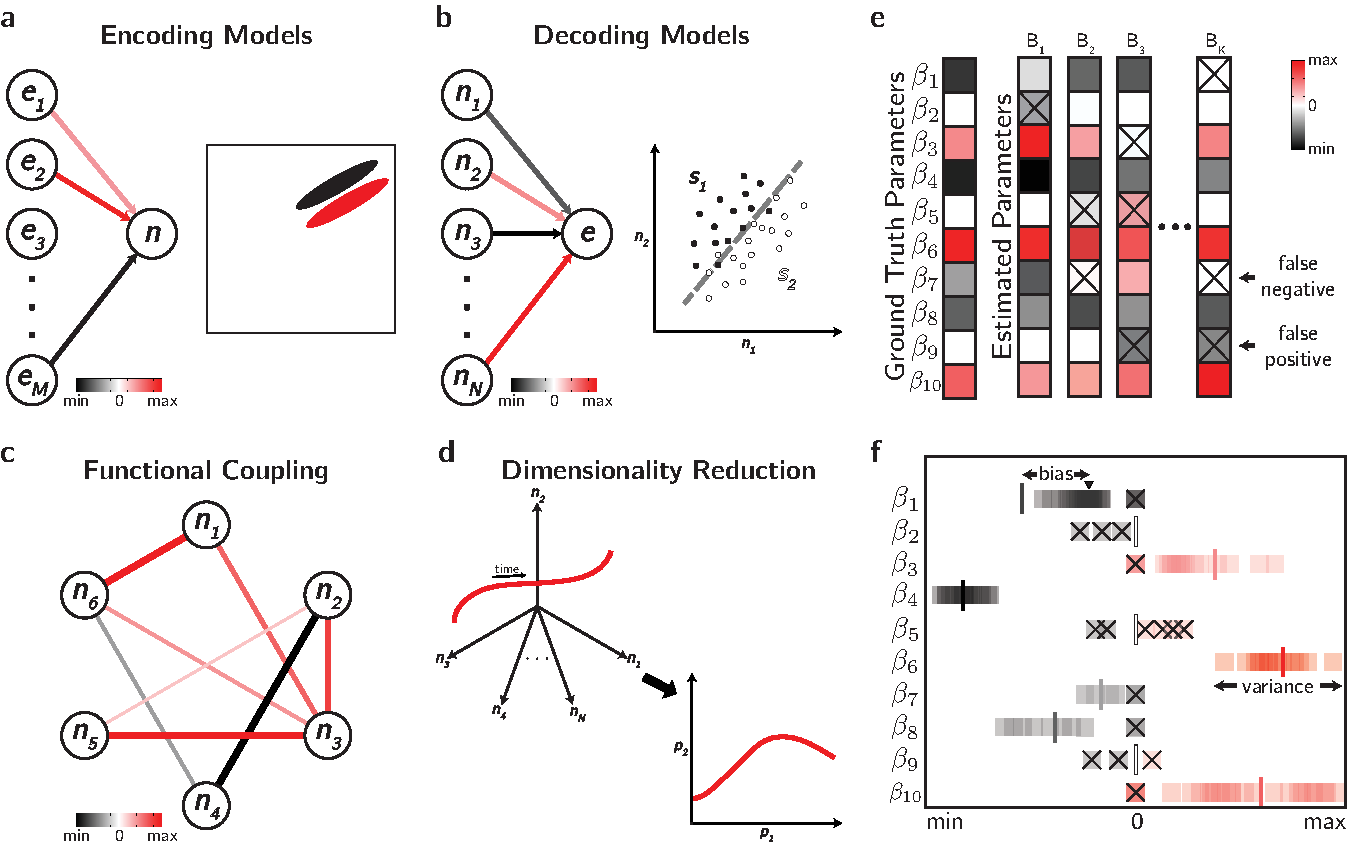
\includegraphics{img/Fig1/Fig1.pdf}}
\caption{{\bf Use cases and assessment of parametric models in neuroscience.}}
\textbf{a} Encoding Models. \textbf{b} Decoding Models. \textbf{c} Functional Coupling. \textbf{d} Dimensionality Reduction \textbf{e} Estimating parameters over bootstraps \textbf{f} Bias and Variance
\end{figure}


\newpage 

\begin{figure}[!htp]
\hspace{-2in}
\scalebox{0.85}{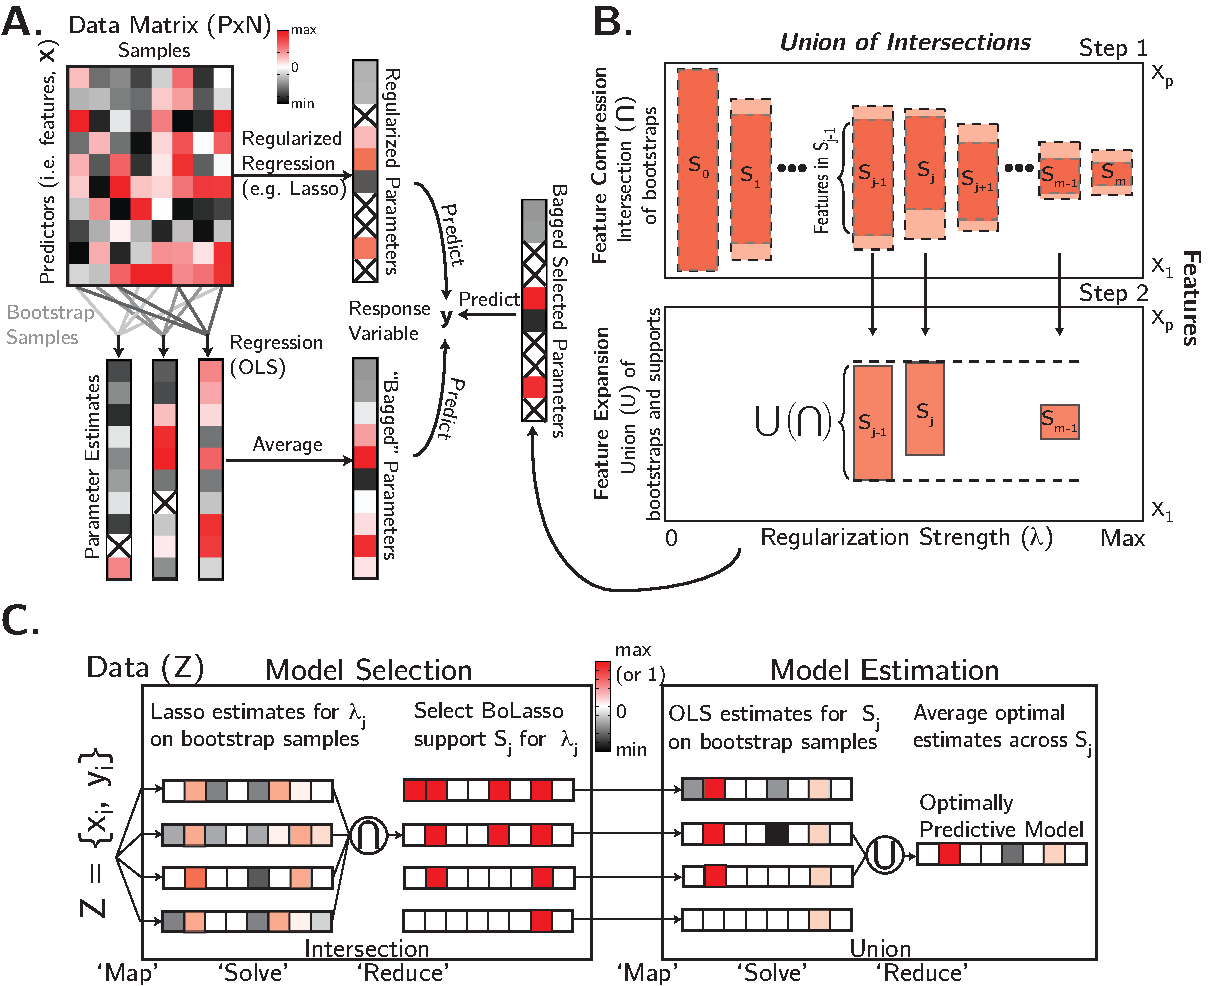
\includegraphics{img/Fig2/Fig2.pdf}}
\caption{{\bf The basic UoI framework.}}
\textbf{a} Schematic of regularization and ensemble methods for regression. \textbf{b} Schematic of the Union of Intersections (UoI) framework. \textbf{c} A data-distributed version of the UoI\textsubscript{Lasso} algorithm.
\end{figure}

\newpage 

\begin{figure}[!htp]
\hspace{-2in}
\scalebox{0.9}{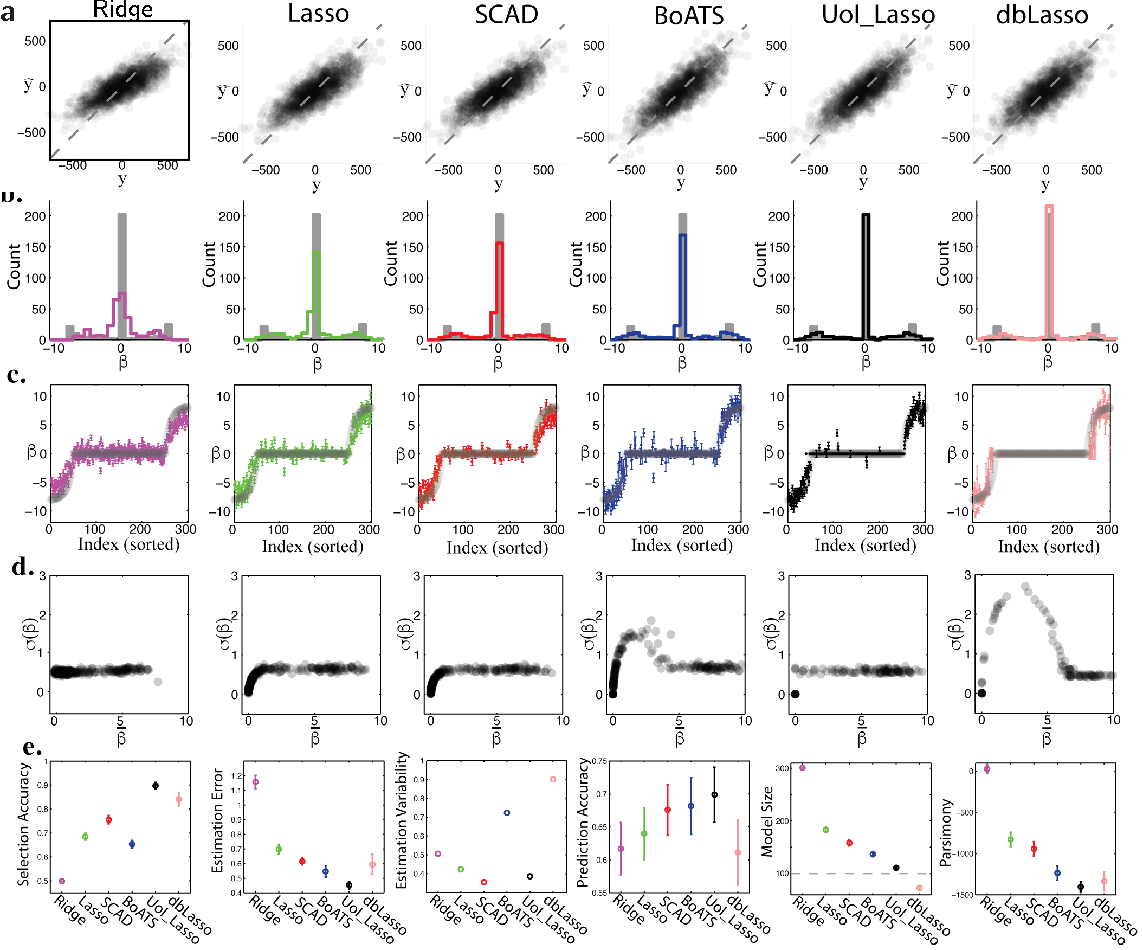
\includegraphics{img/Fig3/Fig3.pdf}}
\caption{{\bf Results on synthetic data.}}
\end{figure}

\newpage


\begin{figure}[!htp]
\hspace{-2in}
\includegraphics{img/Fig5/Fig5.pdf}
\caption{{\bf Coupling Models.}}
\end{figure}


\end{document}

